%* 
%* ------------------------------------------------------------------
%* DispatcherTutorial.tex - Dispatcher Tutorial
%* Created by Robert Heller on Wed May 28 17:16:26 2008
%* ------------------------------------------------------------------
%* Modification History: $Log$
%* Modification History: Revision 1.1  2002/07/28 14:03:50  heller
%* Modification History: Add it copyright notice headers
%* Modification History:
%* ------------------------------------------------------------------
%* Contents:
%* ------------------------------------------------------------------
%*  
%*     Model RR System, Version 2
%*     Copyright (C) 1994,1995,2002-2005  Robert Heller D/B/A Deepwoods Software
%* 			51 Locke Hill Road
%* 			Wendell, MA 01379-9728
%* 
%*     This program is free software; you can redistribute it and/or modify
%*     it under the terms of the GNU General Public License as published by
%*     the Free Software Foundation; either version 2 of the License, or
%*     (at your option) any later version.
%* 
%*     This program is distributed in the hope that it will be useful,
%*     but WITHOUT ANY WARRANTY; without even the implied warranty of
%*     MERCHANTABILITY or FITNESS FOR A PARTICULAR PURPOSE.  See the
%*     GNU General Public License for more details.
%* 
%*     You should have received a copy of the GNU General Public License
%*     along with this program; if not, write to the Free Software
%*     Foundation, Inc., 675 Mass Ave, Cambridge, MA 02139, USA.
%* 
%*  
%* 

\chapter{Dispatcher Tutorial}
\label{chpt:dispatcher:Tutorial}
\typeout{$Id$}

\section{A ``Simple Mode'' CTC Panel}


\begin{figure}[hbpt]
\begin{centering}
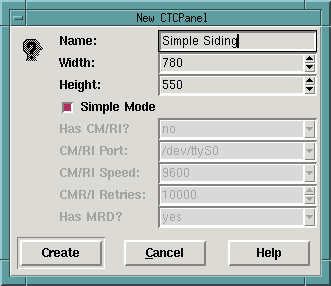
\includegraphics{DISPSimpleTutNewCTC.png}
\caption{Creating a new Simple Mode CTC Panel}
\label{fig:dispatcher:Tut:newSimplePanel}
\end{centering}
\end{figure}
\begin{figure}[hbpt]
\begin{centering}
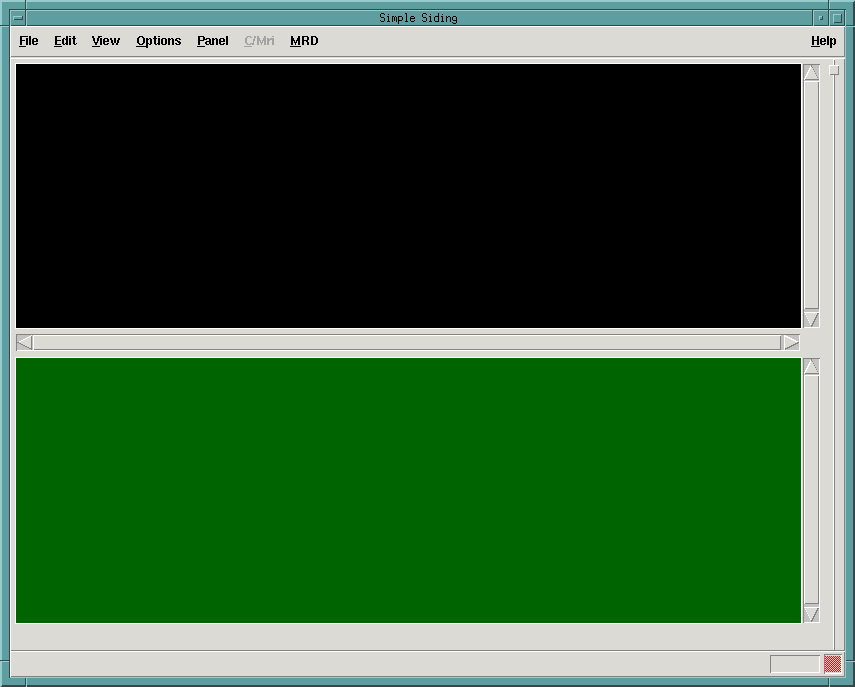
\includegraphics[width=5in]{DISPSimpleTutBlankCTC.png}
\caption{Initial blank panel}
\label{fig:dispatcher:Tut:blankPanel}
\end{centering}
\end{figure}
%
This tutorial will go through the steps of creating a simple CTC panel
for a passing siding.  First, after starting up the Dispatcher program,
we will click on the \texttt{New CTC Window} toolbar button and get a
\texttt{New CTCPanel} dialog box, as shown in
Figure~\ref{fig:dispatcher:Tut:newSimplePanel}. See
Section~\ref{sect:dispatcher:creatingCTCPanels} for more information.
We fill in a name and select the \texttt{Simple Mode} check button.
Clicking on \texttt{Create} gives us the blank panel shown in
Figure~\ref{fig:dispatcher:Tut:blankPanel}. Now we can start adding
track work and control elements.  But first a brief discussion about how
things are structured.  First of all every object has a unique name and
every object is in a named control point.  A ``control point'' is a
collection of track work elements and control panel elements that relate
to a single controlled feature, typically a turnout of some sort. The
control point usually includes a code button, which is a button that
initiates some change in the track work (turnouts, signals, etc.), based
upon the settings of one or more control panel elements.  In this
tutorial we will be creating four control points, \textbf{CP1},
\textbf{CP2}, \textbf{Main}, and \textbf{Siding}.  \textbf{CP1} is the
turnout at the Western (left) end of the siding, \textbf{CP2} is the
turnout at the Eastern (right) end of the siding, \textbf{Main} is the
mainline trackage, and \textbf{Siding} is the siding track. The
\textbf{Main} and \textbf{Siding} control points won't have any control
panel objects and are only being used to contain the simple track
elements. These are essentially ``dummy'' control points and are just
being used as containers for track work that does not contain any
centrally controllable track work.

\begin{figure}[hbpt] 
\begin{centering}
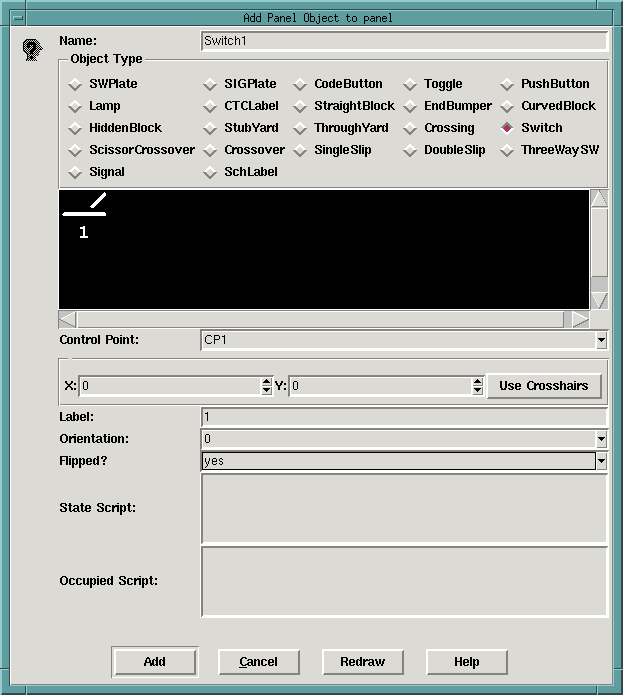
\includegraphics[width=4in]{DISPSimpleTutSw1.png} 
\caption{Creating Turnout 1}
\label{fig:dispatcher:Tut:Sw1} 
\end{centering} 
\end{figure}
%
\begin{figure}[hbpt] 
\begin{centering}
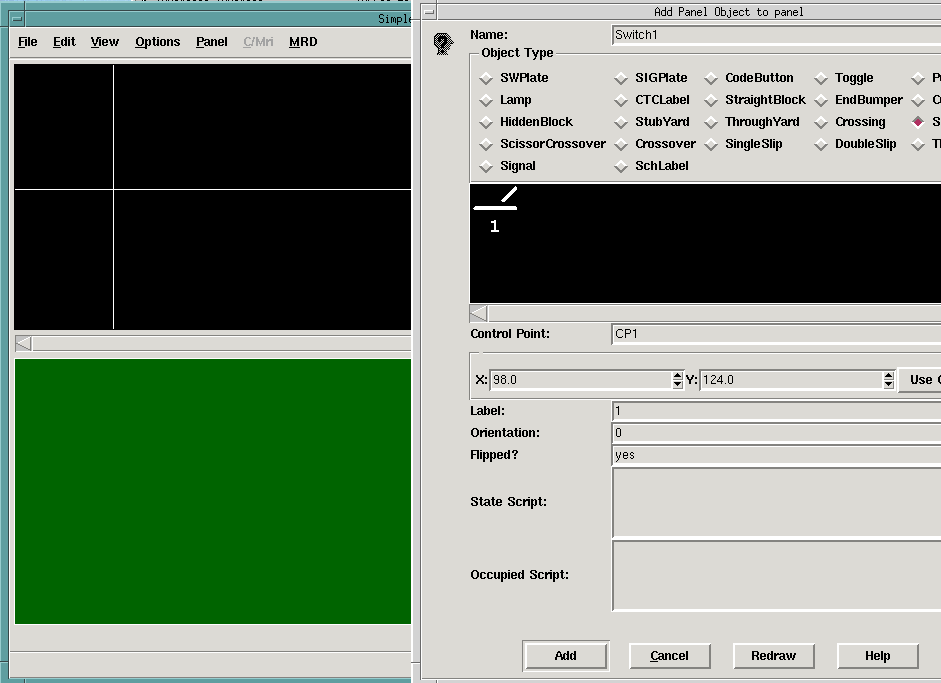
\includegraphics[width=4in]{DISPSimpleTutSw1CrossHairs.png} 
\caption{Positioning Turnout 1} 
\label{fig:dispatcher:Tut:Sw1CrossHairs} 
\end{centering}
\end{figure} 
%
\begin{figure}[hbpt] 
\begin{centering}
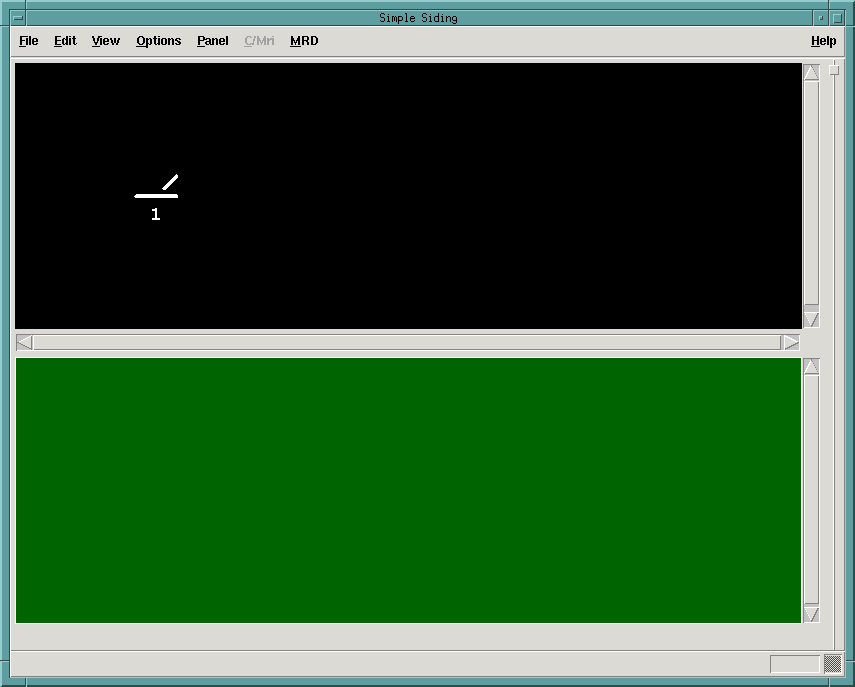
\includegraphics[width=4in]{DISPSimpleTutPanel1.png} 
\caption{Turnout 1 placed on the panel} 
\label{fig:dispatcher:Tut:panel1} 
\end{centering}
\end{figure} 
%
First we will create turnout 1 (named \textbf{Switch1}) by selecting
\texttt{Add Object} on the \texttt{Panel} menu, which gives us the
\texttt{Add Panel Object to panel} dialog box, shown in
Figure~\ref{fig:dispatcher:Tut:Sw1}. See
Section~\ref{sect:dispatcher:addeditdeletePanelElements} for more
information. We will ``flip'' the turnout to give it the proper
orientation. Turnouts can be flipped and can also be rotated to one of
eight positions (45 degree increments). We will use the cross hairs to
roughly position the turnout, as shown in
Figure~\ref{fig:dispatcher:Tut:Sw1CrossHairs}. Clicking the
\texttt{Add} button places the turnout on the track work schematic, as
shown in  Figure~\ref{fig:dispatcher:Tut:panel1}.  \begin{tip}You can
fine tune the location of the object by making small changes to the X
and Y coordinates after you have roughly placed the object using the
cross hairs. You can always go back and edit an object by using the
\texttt{Edit Object} menu item on the \texttt{Panel} menu and then
selecting the name of the object to edit.\end{tip}

\clearpage

\begin{figure}[hbpt] 
\begin{centering}
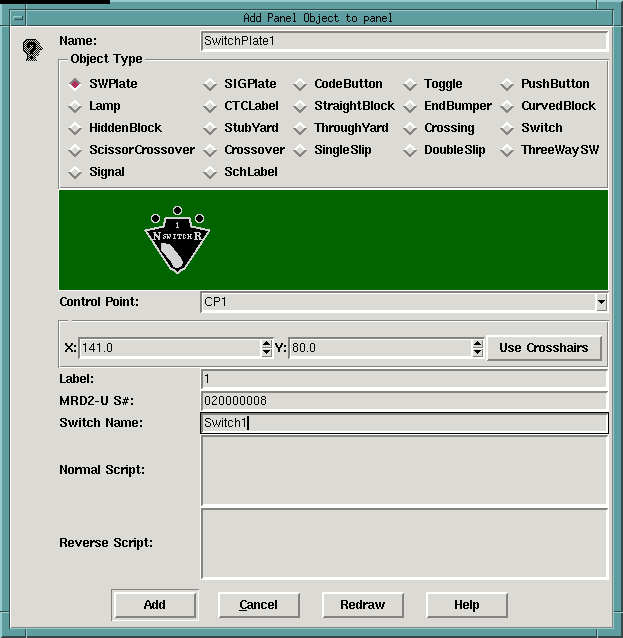
\includegraphics[width=4in]{DISPSimpleTutSWPlate1.png} 
\caption{Adding a Switch Plate} 
\label{fig:dispatcher:Tut:SWPlate1}
\end{centering}
\end{figure} 
%
\begin{figure}[hbpt] 
\begin{centering}
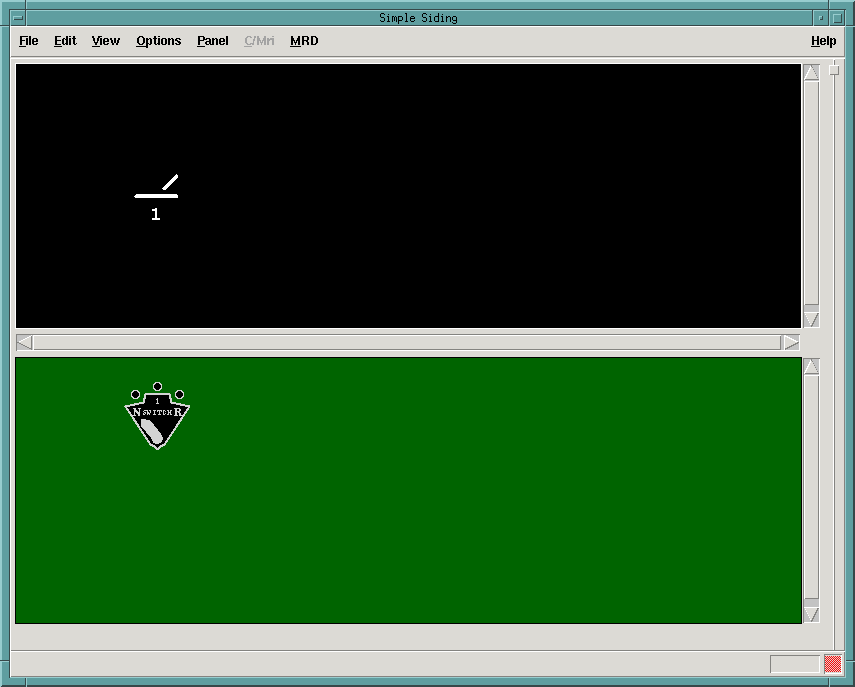
\includegraphics[width=4in]{DISPSimpleTutPanel2.png} 
\caption{Switch Plate 1 placed on the panel} 
\label{fig:dispatcher:Tut:panel2} 
\end{centering}
\end{figure} 
%
Next, we will add a switch plate (named \textbf{SwitchPlate1}), again
by selecting \texttt{Add Object} on the \texttt{Panel} menu, again
using the \texttt{Add Panel Object to panel} dialog box, shown in
Figure~\ref{fig:dispatcher:Tut:SWPlate1}. We will enter the name of the
turnout it controls (\textbf{Switch1}) and the serial number of the
MRD2-U board that will be controlling the Switch-It board powering the
switch motor. Again we will use the cross hairs to place the switch
plate. The result is shown in Figure~\ref{fig:dispatcher:Tut:panel2}.

\clearpage

\begin{figure}[hbpt] 
\begin{centering}
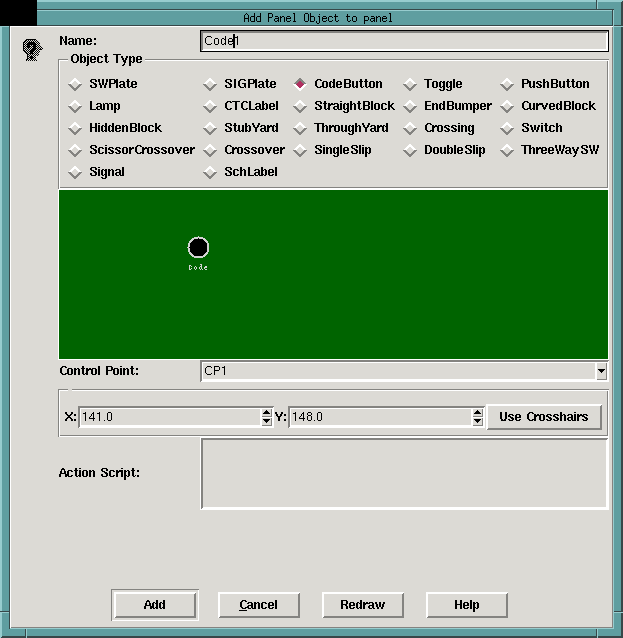
\includegraphics[width=4in]{DISPSimpleTutCB1.png} 
\caption{Adding a code button} 
\label{fig:dispatcher:Tut:CB1}
\end{centering}
\end{figure} 
%
\begin{figure}[hbpt] 
\begin{centering}
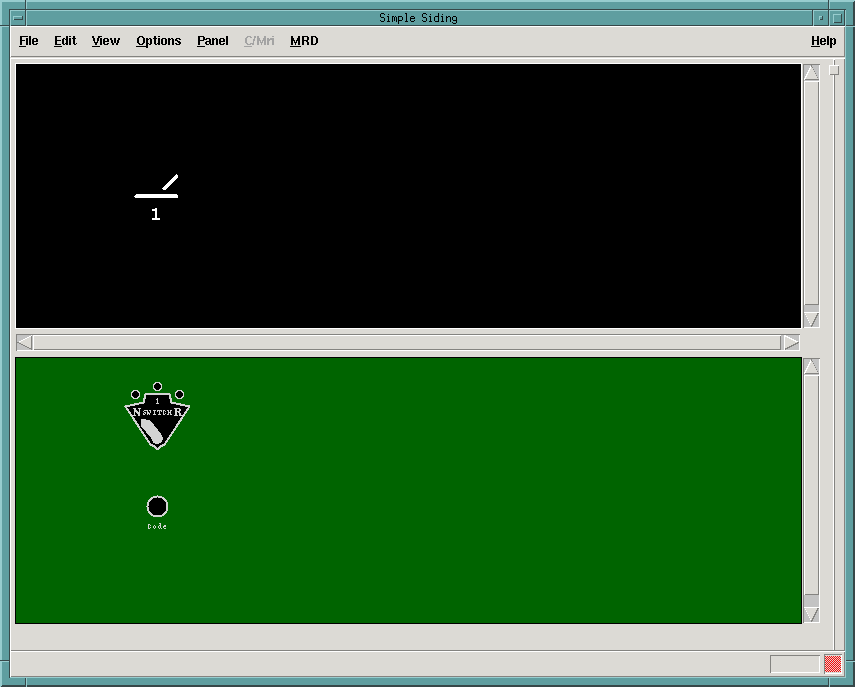
\includegraphics[width=4in]{DISPSimpleTutPanel3.png} 
\caption{Code button 1 placed on the panel} 
\label{fig:dispatcher:Tut:panel3} 
\end{centering}
\end{figure} 
%
Finally, we will add a code button, as shown in
Figures~\ref{fig:dispatcher:Tut:CB1} and
~\ref{fig:dispatcher:Tut:panel3}.

\clearpage

\begin{figure}[hbpt] 
\begin{centering}
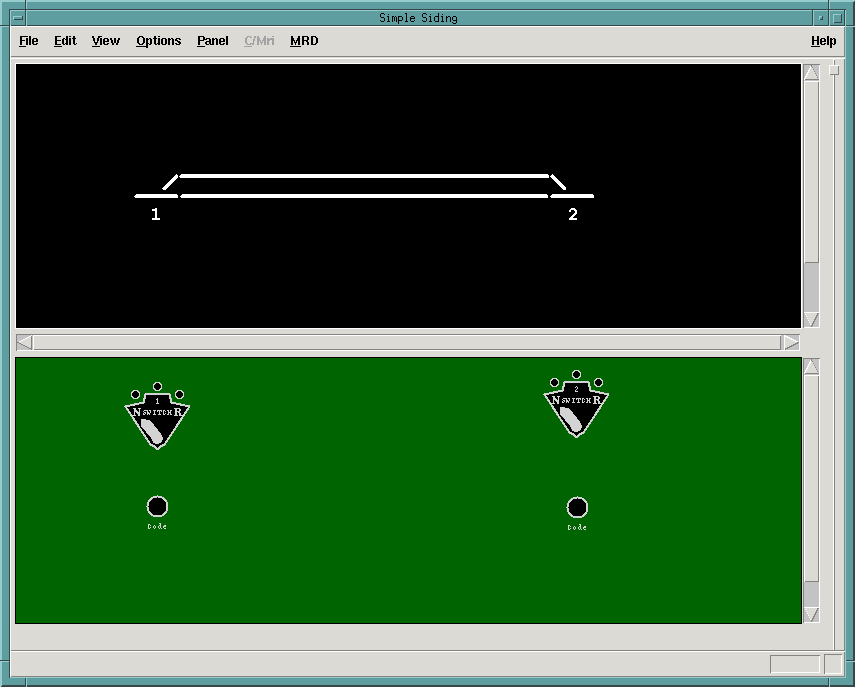
\includegraphics[width=5in]{DISPSimpleTutPanel4.png} 
\caption{The completed panel} 
\label{fig:dispatcher:Tut:Panel4} 
\end{centering}
\end{figure} 
%
We repeat this process to add the mainline, the siding, and the second
turnout, with its switch plate and code button. \begin{tip}Place the
second turnout next, then add the mainline and the siding tracks. Once
the turnouts have been placed, the locations of the endpoints of the
straight track sections are easy to select.\end{tip} Finally we get the
panel shown in Figure~\ref{fig:dispatcher:Tut:Panel4}.

Once the panel has been completed, we can use the \texttt{Wrap As} menu
item under the \texttt{File} menu to create a ``wrapped'' version of
the generated program.  This is a self-contained, stand-alone
executable program that implements the CTC panel. See
Section~\ref{sect:dispatcher:wrapas} for more information.



%%\section{A more advanced Example}
